\begin{quotation}
{\footnotesize
\noindent{\emph{``In math, you're either right or you're wrong.''\\}
}
\begin{flushright}
Katherine Johnson
\end{flushright}
}
\end{quotation}
\vspace{0.5cm}

\section{Mathematical Preliminaries}

\subsection{Reference Frames}
In order to be able to correctly analyze to problem of image generation, five reference frames are of interest:
\begin{itemize}
\item \acrfull{gci}
\item chaser body-fixed frame
\item camera frame
\item target model frame
\item target body-fixed frame
\end{itemize}

The \acrshort{gci} frame has its origin at the center of mass of the Earth. This frame has a linear acceleration because of the Earth's circular orbit about the Sun, which however can be neglected for attitude analysis.
It's axes are aligned with the mean North pole and the mean vernal equinox at some epoch.\\
The chaser and target body-fixed frames have their origins at the \acrshort{cg} of both, respectively, and their axes are usually aligned with their respective principal axes.
The origin of the camera frame instead coincides with the center of perspective projection.\\
The target model frame is fixed with respect to the body frame and often coincides with it.\\
For what concerns this work, we will consider the camera frame to be coincident with the chaser body-fixed frame, and the target model frame to be coincident with the target body-fixed frame.\\
The transformation from one reference frame to another can be uniquely defined by means of a translation vector and a rotation matrix. The translation vector represents the relative positions between the two different frames origins and the rotation matrix is determined by a sequence of three rotations about three different linearly independent axis by three angles, according to the Euler's angle representation.


\section{Image generation}
The use of artificial images gives a complete control over the scene.\\
As stated in \cite{paolocorti}, the generated dataset should be as complete as possible in terms of metals and terrain features and illumination conditions.\\
A lack of realism in image generation can lead to incoherent results, not representative of real operative conditions and thus can lead to wrong results in terms of \acrshort{cv} algorithm tuning.\\
A particular care is then required in the image generation process.\\
For the purpose of this work, a new procedure for the generation of realistic images, representative of a dataset taken by a monocular navigation camera during a close-proximity approach to targeg \acrshort{sc} has been developed.\\
Unsing the illustrated procedure, the user is able to create synthetic images of a target \acrshort{sc} given it's \acrshort{stl} model, by fine tuning all the properties of the materials composing the target \acrshort{sc}.\\
Since there could be also cases in which the Earth can be behind the target \acrshort{sc}, the developed tool is also able to simulate Earth's presence at any given location. The tool is also able to the simulate the the athmosphere of the Earth and the cloud layer \cite{jacopo}.\\
The developed tool couples a well known open source raytracer (\acrshort{povray}) with MATLAB in order to archive a good degree of realism in the generated images.\\

\subsection{Ray Tracing}
\subsubsection{What is ray tracing}
Ray tracing is a rendering technique used for generating artificial images which relies on the concept of controlling the path of view lines which starts from the observer camera and ends to generic virtual objects and thus calculating the color of the object.
What is really of crucial importance for our particular use case is that ray tracing is capable of re-creating some of nature's optical effects through transparent and opaque surfaces as reflection and refraction, scattering, and dispersion phenomena (such as chromatic aberration).
Due to this, ray tracing techniques can generate artificial images with a really high degree of photorealism.
When the ray tracer renders the scene, a ray of light is traced for every pixel of the camera. Typically, each ray must be tested for intersection with some subset of the object in the scene. Once the ray has intercepted an object, the ray tracing algorithm will estimate the amount and the type of incoming light at the point of intersection, examine the material properties declared by the programmer and by combining those information will calculate the final color that should be attributed to the pixel.
Several illumination algorithms and reflective or translucent materials may also require more rays to be re-cast into the scene in order to do the necessary computations.
At first glance may seem cumbersome to start the ray from the observer towards the object rather than casting rays to the camera (as is in reality). However, doing so speeds up a lot the computation time, as most of the light rays present in a scene may never reach the eye of the observer, and so, all the time spent for tracing those would be useless.
After either a maximum number of reflections or a ray traveling a certain distance without intersection, the ray ceases to travel and the pixel's value is updated.\\

\begin{figure}[H]
\centering
\includegraphics[width=0.85\textwidth]{gfx/scherma-ray-tracing.eps}
\caption{Raytracing: from the observer to the light source \cite{pictraytracing}}
\label{fig:raytracing}
\end{figure}

For more information regarding how ray tracing works, and ray tracing techniques see  \cite{introductionraytracing}.

\subsubsection{Ray tracing with \acrshort{povray}}
\acrshort{povray} gives the programmer several options to customize both the look and feel and the optical properties of the represented objects and the medium that light passes trough.\\
\acrshort{povray} offers the programmer the choice to use some predefined geometric shapes, like spheres or cubes; another option instead is to define surfaces of the objects trough meshes. This capability has been used widely by this project to model the spacecraft object.\\
Any surface can then be characterized by its own optical properties. Every object can have a color specified by an RGB triplet or can be wrapped with a texture.\\
The light source is not really an object. Light sources have no visible shape of their own. They are just points or areas which emit light and can be tuned to accomplish the wanted result, for example we can tune the intensity of the light and the light color by specifying the RGB triplet; any atmospheric effect like opaque gas presence (like smoke or clouds) and its rlative optical distortions can be modeled as well.\\

\subsection{Environment Modeling}
\subsubsection{Earth Modeling}
Earth modeling has been worked out in collaboration with Jacopo Guarneri.
Here will follow a brief review of how Earth has been modeled taken from \cite{jacopo}.\\
For modeling the Earth, the \acrshort{povray} \inlinecode{POV}{sphere} object has been used, in conjunction with the \inlinecode{POV}{scale} feature, which allows to make the sphere become an ellipsoid.

\begin{figure}[H]
\centering
\includegraphics[width=0.85\textwidth]{gfx/sphere_scaling.eps}
\caption{Sphere manipulation with \acrshort{povray} \cite{jacopo}}
\label{fig:spherescaling}
\end{figure}

Once the \acrshort{3d} object is created, the most natural choice one can think of is to wrap a \acrshort{2d} texture of the Earth (\ref{fig:firstTexture}) on it, and this indeed is what has been done, using the high resolution (8K) texture of the Earth.

\begin{figure}[H]
\centering
\includegraphics[width=0.85\textwidth]{gfx/first_text.eps}
\caption{Initially chosen texture of the Earth}
\label{fig:firstTexture}
\end{figure}

\bigskip

In \ref{fig:EarthApollo} we can see a comparison of the synthetically generated image and an actual true image of the Earth as seen from the Apollo 11. From a first glance, used texture gives a good representation of what we should see when we look of a picture of the Earth taken from the space. 

\begin{figure}[H]
\centering
\includegraphics[width=0.85\textwidth]{gfx/earthApolloOurs.eps}
\caption{Comparison of synthetic Earth image with Apollo 11's picture}
\label{fig:EarthApollo}
\end{figure}

Despite the relatively good result, this way of modeling the Earth still haves some issues : 
\begin{itemize}
\item since for all pictures we use the same texture, the clouds are sticked to their position on top of the surface of the Earth;
\item there is no way to define different optical properties for the terrain and the seas;
\item there is no way to try to simulate diffusion of sunlight in the atmosphere;
\end{itemize}
In the following, those issues will be addressed.

\paragraph{Cloud Layer}\mbox{}\\
The fixed coupling of Earth surface and clouds is big problem for what concerns CV algorithms development, which should be trained to work in several different conditions, so, having the clouds always on the same region of the Earth despite the orientation is not acceptable.\\
The solution adopted in both this work and \cite{jacopo} relies on decoupling the Earth terrain layer and the cloud layer, specifying different optical properties for each layer, specify clouds relative rotation with respect to the terrain and coupling back everything together. 
Furthermore, oceans have been splitted too, in order to be able to set different optical properties for the seas.\\
For the terrain layer, a a true-color mercator image of the Earth has been used as a base, in this way every piece of the surface could possibly be visible in any picture.

\begin{figure}[H]
\centering
\includegraphics[width=0.85\textwidth]{gfx/earthMercator.eps}
\caption{True Color Earth Mercator Image \cite{bluemarble}}
\label{fig:EarthMercator}
\end{figure}

\bigskip

As said before, in order to be able to use different optical properties for water and terrains, a separate two-color mercator-projection image of the Earth where the water is black and the land is white has been used.

\begin{figure}[H]
\centering
\includegraphics[width=0.85\textwidth]{gfx/landmask_mercator.eps}
\caption{Landmask Mercator Image}
\label{fig:LandmaskMercator}
\end{figure}

\bigskip

In \ref{fig:comparisonEarths} the result of differentiating the optical properties for terrains and oceans is shown. Despite the fact that it may seems that there is only a small distinction between the two images (in particular, shinier oceans and darker forests), is still enough the make the Earth to seem more photorealistic, and it leave some space for further tuning.

\begin{figure}[H]
\centering
\includegraphics[width=0.82\textwidth]{gfx/comparisonEarths.eps}
\caption{Comparing images with no differential treatment between land
and ocean and with differential treatment}
\label{fig:comparisonEarths}
\end{figure}

\bigskip

The cloud layer is added on top of the cloudless surface and thanks to that, it can rotate with respect to the Earth by a prescribed angle set by the programmer. The cloud layer texture and the shape of the clouds itself always remains the same, but this can be partially mitigated by using different cloud textures.

\begin{figure}[H]
\centering
\includegraphics[width=0.85\textwidth]{gfx/clouds.eps}
\caption{Two-color mercator image of Earth's cloud layer}
\label{fig:cloudsMercator}
\end{figure}

\bigskip

The cloud texture used for this work (\ref{fig:cloudsMercator}) is not actually directly printed on the surface of the earth, but rather is extruded on a shell built around the sphere which defines the Earth, which has an inner radius equal to $R_{in} = 1.001 \cdot R_{Earth}$ and an outer radius equal to $R_{out} = 1.0002 \cdot  R_{Earth}$. Those values have been found by taking as a reference the fact that low Earth clouds ranges from an altitude of \SI{600}{\m} to \SI{15000}{\m} \cite{nimbostratus}. Although higher or thicker clouds can be modeled, this will require longer rendering times. Of course, also for the cloud layer is possible to set custom optical properties, in order to make the clouds partially transparent, so that when there isn't a dense cloud area, the terrain behind is still visible under the white blanket.\\ 
The result of adding the cloud layer can be seen in \ref{fig:cloudShell}

\begin{figure}[H]
\centering
\includegraphics[width=0.82\textwidth]{gfx/cloudShell.eps}
\caption{Earth's representation using cloud shell}
\label{fig:cloudShell}
\end{figure}

\paragraph{Cloud Layer}\mbox{}\\
Recreating the characteristic atmosphere presence around the Earth is of crucial importance for developing a CV algorithm for space applications, as it is needed in order to train the algorithm itself to work into a real-case scenario.
The atmosphere's presence in fact would enlarge the aspect of the Earth in the image, and furthermore would stress the edge detection algorithms.
To recreate the atmospheric shine effect, a strategy which is similar to the one adopted to model the cloud layer has been used. In fact, it has been modeled as a shell with a certain thickness of a transparent material with some scattering properties.
For what concerns both this project and what has been done in \cite{jacopo}, the gaseous layer was made only \si{25}{km} thick. Despite the fact that the atmosphere should be visible up to many more kilometers, the computational load introduced by rendering a much high atmosphere is not negligible on a standard PC hardware, and so the image generation time would grow up exponentially, making the task of compiling a data-set of thousands of images very time consuming.
In figure \ref{fig:earthAtmo} can be seen the final result of adding the atmospheric model.\\

\begin{figure}[H]
\centering
\includegraphics[width=0.82\textwidth]{gfx/earthFinal.eps}
\caption{Earth with the atmosphere layer}
\label{fig:earthAtmo}
\end{figure}

\bigskip

In figure \ref{fig:trueVsFake} instead is possible to view the artificially generated next to a real Earth picture taken by NASA's Suomi NPP on January 4, 2012.
It can be seen that, despite the fact that the real image isn't perfectly reproduced (because some other factors should be known in order to be taken into account, such as exposure time), the synthetic image still provide an high degree of similarity with the real one.

\begin{figure}[H]
\centering
\includegraphics[width=0.82\textwidth]{gfx/trueVsFake.eps}
\caption{Comparison between true and final rendered Earth image}
\label{fig:trueVsFake}
\end{figure}

In table \ref{tab:EarthParameters} are briefly resumed the values used to model the various layer of the Earth.

\begin{table}[H]
\centering
\begin{tabular}{c cccc}
\hline 
\hline
 & Terrain & Oceans & Clouds & Atmosphere \\ 
\hline 
Ambient & 0.001 & 0.001 & 0.001 & 0.0001 \\ 
Roughness & 0.05 & 0.1 & 0.005 & 0.5 \\ 
Brillance & 1 & 1 & 1 & 1 \\ 
Diffuse & 0.85 & 0.85 & 1 & 0.6 \\ 
Reflection & 0 & {0.04, 0.25} & 0 & 0 \\ 
Specular & 0 & 0.1 & 0 & 0 \\ 
\hline
\hline
\end{tabular}
\caption{Optical parameters of Earth's different layers}
\label{tab:EarthParameters} 
\end{table}

\subsubsection{Light Modeling}
For an object to show up into the scene, it must be illuminated.
There are two ways to illuminate an object with \acrshort{povray}:

\begin{itemize}
\item use a standard light source
\item use ambient light
\end{itemize}

The light source is controlled by the keyword \inlinecode{POV}{light_source}, which in turn accepts several modifiers. Light sources in \acrshort{povray}have no visible shape of their own. They are just points or areas which emit light.\\
The ambient light instead is controlled by the keyword \inlinecode{POV}{ambient} added to the \inlinecode{POV}{finish} modifier of an object, and it is used to simulate the light inside a shadowed area.
We can think of ambient light like a kind of light that is scattered everywhere in the room. It bounces all over the place and manages to light objects up a bit even where no light is directly shining.
In our particular case, we can use the \inlinecode{POV}{ambient} option to simulate the illumation of the object due to spurious light sources (such as stars) or reflection from other bodies (like the Moon or other planets).
In order to model the lightning condition of a true solar system, the light source has been modeled to resemble as much as possible the light emitted by the Sun.
The solution adopted in this project and in \cite{jacopo} relies upon modeling the sun as an area light source through the option \inlinecode{POV}{area_light}. This allows to create a cluster of point-like light sources distributed on a disc (simulated by adding the \inlinecode{POV}{circular} option to the area light source) which has radius equal to the radius of the Sun, and placed at the exact distance which the Sun has from the Earth in the \acrshort{gci} frame. In order to cope with the fact that in reality the Sun is equal to a sphere of light and not a disc, the option \inlinecode{POV}{orient} has been used. When using \inlinecode{POV}{orient}, every object in the \acrshort{povray} world would see the Sun's disc as oriented toward it, from any position around it.
Furthermore, the option \inlinecode{POV}{jitter} has been used, which tells the ray-tracer to slightly move the position of each light in the area light to eliminate any shadow banding that may occur.

\subsection{Tango Spacecraft Modeling}
% copia un po franchiolla e un po il paper, devi solo dirgli come è fatto il satellite

\subsubsection{3D Model of the Spacecraft}
The problem of modeling rather complex shapes with \acrshort{povray}, such as can be a spacecraft, it was one of the most long and painful one during this work, which also required to patch \acrshort{povray} source code, to prevent the ray-tracer to made assumption that aren't true.
Obviously, the path of building the \acrshort{sc} using \acrshort{povray} primitives was really not feasible, as many different \acrshort{sc} can have different shapes, and modeling them by using simpler shapes it is simply not possible. Furthermore, usually detaled \acrshort{3d} CAD models of \acrshort{sc} are available which can be easily exported into \acrshort{stl} format, so the focus has been putted into trying to understand how to translate those \acrshort{3d} CAD models directly into \acrshort{povray} code.\\
Several open source and closed source software have been coupled together in order to produce trough \acrshort{povray} a render of a given \acrshort{stl} model.
The procedure will be detailed in the following paragraphs.
The Tango spacecraft has been modeled using the dimensions specified in \cite{Sharma2018}, which will be here reported for ease of reading. The solar panel is represented by a polygon of \si{570}{mm} x \si{759}{mm}, while the spacecraft body instead is represented by a convex polyhedron of \si{560}{mm} x \si{550}{mm} x \si{300}{mm}. The radio frequency antennas length instead is of \si{204}{mm}. The origin of the CAD model is located in correspondence of the \acrshort{cg}.\\
Using the aforementioned dimensions, the Tango spacecraft has firstly been reproduced using Autodesk Inventor. The result of the modeling procedure is shown in figure \ref{fig:tango3d}.
\begin{figure}[H]
\centering
\includegraphics[width=0.62\textwidth]{gfx/tangoScreenshot2.eps}
\caption{Tango \acrshort{sc} \acrshort{3d} model}
\label{fig:tango3d}
\end{figure}
The \acrshort{3d} CAD model can now be exported in \acrshort{stl} format to be manipulated through other software.

\subsubsection{Blender}
Once the \acrshort{3d} model of the Tango \acrshort{sc} was available, the most challenging task has been the one of rendering the \acrshort{sc} itself using \acrshort{povray} at attitudes imposed by the user.\\
The first step for archiving that goal is to import the \acrshort{stl} model of the \acrshort{sc} into Blender.\\
By exploiting the \acrshort{povray} render add-on for Blender, it is possible to render any given \acrshort{stl} file imported file using \acrshort{povray} as rendering engine. The \acrshort{povray} add-on will optionally save the generated SDL code used to render the scene.\\
The generated code however, will threat the entire \acrshort{3d} model as a whole, generating one giant \acrshort{povray} \inlinecode{POV}{mesh2} object, which is something which cannot be easily managed. Just as an example, would be impossible to assign to the different parts of the \acrshort{sc} different optical parameters or textures.\\
So, to workaround this limitation, it is a good practice to first split the different surfaces of the \acrshort{3d} model in different different children objects (or children surfaces), and only after render the scene in order to get the POV code. In that way, the \acrshort{povray} render add-on for Blender will generate a \inlinecode{POV}{mesh2} object for each children object created in Blender.
This will enable us to set different material properties for each children surface or to apply different textures to different surfaces.
For the purpose of this work, the original \acrshort{stl} model has been subdivided into thirty children object, each one with its own optical parameters, as can be seen from figure \ref{fig:tangoblender} .

\begin{figure}[H]
\centering
\includegraphics[width=0.82\textwidth]{gfx/tangoBlender.eps}
\caption{Tango \acrshort{sc} \acrshort{3d} model in Blender}
\label{fig:tangoblender}
\end{figure}

The Blender \acrshort{povray} add-on also let the user to inject custom POV code (figure \ref{fig:tangoblenderpov}) into the auto-generated one, which can be useful especially for adding textures, for example to the solar panels, as it has been done into this project.

\begin{figure}[H]
\centering
\includegraphics[width=0.82\textwidth]{gfx/tangoBenderPOVCode.eps}
\caption{Add custom POV code into Blender}
\label{fig:tangoblenderpov}
\end{figure}

The end results is showed in figure \ref{fig:tangoblenderfinal}

\begin{figure}[H]
\centering
\includegraphics[width=0.82\textwidth]{gfx/tangoPolished.eps}
\caption{Tango \acrshort{sc} rendered using \acrshort{povray} Blender add-on}
\label{fig:tangoblenderfinal}
\end{figure}

\subsubsection{\acrshort{povray}}
The major issue of the code generated from the  \acrshort{povray} Blender add-on is that is composed of several separated \inlinecode{POV}{mesh2} objects which makes almost impossible to rotate the whole object by imposing a given attitude matrix, since one is supposed to rotate all the \inlinecode{POV}{mesh2} objects by hand.\\
In order to workaround this limitation, from all the \inlinecode{POV}{mesh2} objects which have been generated from \acrshort{povray} Blender add-on are merged into one single \inlinecode{POV}{merge} object.
The \inlinecode{POV}{merge} \acrshort{povray} operation allows to bind two or more shapes into a single entity that can be manipulated as a single object, which is exactly what we want. The new object created by the merge operation can be scaled, translated and rotated as a single shape. The entire merge can share a single texture and optical parameters but each object contained in the union may also have its own texture and optical parameters, which will override any texture statements in the parent object. So, all the \inlinecode{POV}{mesh2} objects which describes the \acrshort{sc} surfaces are merged into a single big (21K LoC) \textbf{spacecraft} \inlinecode{POV}{merge} object. \\
To ease the usage of the \inlinecode{POV}{merge} object, a \acrshort{povray} include file it is created, with the sole purpose of containing the \textbf{spacecraft} \inlinecode{POV}{merge} object.
The include file is read in as if it were inserted at that point in the file. Using include is almost the same as cutting and pasting the entire contents of this file into the scene. This allow to define the \textbf{spacecraft} \inlinecode{POV}{merge} once and call it from any other POV file just like any other predefined object is called, and so, it is possible to manipulate its position and orientation in a much more easier way.\\
In table \ref{tab:SCParameters} are briefly resumed the optical parameters used to model the different part of the \acrshort{sc}.

\begin{table}[H]
\centering
\begin{tabular}{c cccc}
\hline 
\hline
 & Solar Panels & Antennas & Main Body \\ 
\hline 
Ambient & 0.0 & 0.25 & 0.25 \\ 
Roughness & 0.13 & 0.0005 & 0.0005 \\ 
Brillance & - & 3.15 & 3.15 \\
Diffuse & 0.3 & 0.95 & 0.99 \\ 
Reflection & {0.23, 0.5} & {0.65, 1} & {0.65, 1} \\ 
Specular & 0.04 & 0.96 & 0.96 \\
Phong & - & 0.43 & 0.43 \\
Phong Size & - & 25 & 25 \\
\hline
\hline
\end{tabular}
\caption{Optical parameters of \acrshort{sc} different parts}
\label{tab:SCParameters} 
\end{table}

\subsection{Camera Modeling}
In \acrshort{povray}'s camera environment, the programmer can set all relevant camera parameters, which will be then used to simulate the camera trough which the scene will be rendered.\\
The most meaningful parameters which can be modeled are the \inlinecode{POV}{location}, the \inlinecode{POV}{direction} of the boresight axis (where is the
camera looking at with \inlinecode{POV}{look_at}), the view angle and the direction of the camera reference frame (by using \inlinecode{POV}{up} and \inlinecode{POV}{right} keywords).\\
The major issue which has been faced when modeling the camera in \acrshort{povray} is the fact that the program defaults to a left handed coordinate system to describe the scene, while all other software (like Autodesk Inventor, Blender) are using a right handed coordinate system.

\begin{figure}[H]
    \centering
        \subfloat[]{\includegraphics[width=0.4\textwidth]{gfx/povrayTern.eps}}
        \qquad
        \subfloat[]{\includegraphics[width=0.4\textwidth]{gfx/povrayHand.eps}}
        \caption{\acrshort{povray} coordinate system}
    \label{fig:povraycoordinatesystem}
\end{figure}

Moreover, the right handed coordinate system is used also to model the orbit that the spacecraft will follow and the spacecraft attitude from Euler equations.\\
It is possible to trick \acrshort{povray} to behave like it using a right handed coordinate system by acting on the \inlinecode{POV}{right} vector of the camera environment. The camera \inlinecode{POV}{right} vector describes the direction to the right of the camera, so, in practicte, tells \acrshort{povray} where the right side of the screen is. Therefore, the  sign of the x component of the \inlinecode{POV}{right} vector can be used to determine the handedness of the coordinate system in use.\\

\begin{figure}[H]
    \centering
        \subfloat[]{\includegraphics[width=0.4\textwidth]{gfx/axesLeft.eps}}
        \qquad
        \subfloat[]{\includegraphics[width=0.4\textwidth]{gfx/axesRight.eps}}
        \caption{Right Handed Coordinate System and Left Handed Coordinate System}
    \label{fig:frames}
\end{figure}

By default \acrshort{povray} use a positive x value in the \inlinecode{POV}{right} vector. This means that the right side of the screen is aligned with the +x-direction. By using a negative x value in the \inlinecode{POV}{right} vector instead the right side of the screen will be aligned to the -x-direction, and the coordinate system will be right handed.\\
Doing only that however left us having the y axis as the one pointing upward and the z axis as the one point in the direction which goes outside the screen.\\
To have a more comfortable, which also uses the same axes of the \acrshort{gci} reference frame, we can flip y and z axis by overriding the \inlinecode{POV}{sky} vector.
By default, in fact, \acrshort{povray} uses \inlinecode{POV}{<0,1,0>} as \inlinecode{POV}{sky} vector. By redefining it as \inlinecode{POV}{<0,0,1>}  \acrshort{povray} will roll the camera until the top of the camera is in line with the sky vector, giving us the desired result.

\begin{figure}[H]
    \centering
        \subfloat[]{\includegraphics[width=0.4\textwidth]{gfx/tangoAxesNormal.eps}}
        \qquad
        \subfloat[]{\includegraphics[width=0.4\textwidth]{gfx/tangoAxesAfterRight.eps}}
        \qquad
        \subfloat[]{\includegraphics[width=0.4\textwidth]{gfx/tangoAxesSky.eps}}
        \caption{Right Handed Coordinate System and Left Handed Coordinate System}
    \label{fig:framesComparison}
\end{figure}

In order to rightly simulate a real camera, the \acrshort{povray} camera aperture angle has been computed by assuming the intrinsic properties of a real camera, a Point Grey Grasshopper 3, equipped with a Xenoplan 1.9/17 mm lens, which is the same camera employed to capture the SPEED dataset \cite{DBLP:journals/corr/abs-1911-02050}.

\begin{table}[H]
\centering
\begin{tabular}{ccc}
\hline 
\hline
Parameter & Description & Value \\ 
\hline 
$N_u$ & Number of horizontal pixels & 1920 \\ 
\hline 
$N_v$ & Number of vertical pixels & 1200 \\ 
\hline 
$f_x$ & Horizontal focal length &  \SI{17.6}{\mm} \\ 
\hline 
$f_y$ & Vertical focal length &  \SI{17.6}{\mm} \\ 
\hline 
$d_u$ & Horizontal pixel length &  \SI{5.86e-3}{\mm} \\ 
\hline 
$d_v$ & Vertical pixel length &  \SI{5.86e-3}{\mm} \\ 
\hline 
\hline
\end{tabular} 
\caption{Parameters of the camera used to capture the SPEED images \cite{DBLP:journals/corr/abs-1911-02050}}
\label{tab:SPEEDCameraParameters} 
\end{table}

By assuming a \acrshort{ccd} sensor which only has square pixels we can obtain:

\begin{equation}
A. R. = \frac{N_u}{N_v}
\end{equation}

\begin{equation}
CCD_{size} = d_u \cdot N_u
\end{equation}

\begin{equation}
\alpha = 2 \cdot \arctan{\frac{CCD_{size}}{2 \cdot f_x}}	
\end{equation}

where $A.R.$ is the Aspect Ratio of the picture, which is passed as first component \inlinecode{POV}{right} vector (with the negative sign, as described before), and $\alpha$ is the aperture angle which will be input in \acrshort{povray}.
Using the parameters detailed in table \ref{tab:SPEEDCameraParameters} we can compute:
\begin{itemize}
\item $A.R.$ = $1.6$
\item $\alpha$ = $35.4515 ^{\circ}$
\end{itemize}

\begin{figure}[H]
\centering

\includegraphics[width=0.82\textwidth]{gfx/tangoNoNoise.eps}
\caption{Tango \acrshort{sc} rendered using table \ref{tab:SPEEDCameraParameters} parameters}
\label{fig:tangoNoNoise}
\end{figure}

\subsection{Adding the noise}
Finally, for augmenting the "realness" of an image generated though \acrshort{povray}, the image needs to be post-processed using MATLAB.
The image so is input in MATLAB and two different noises are applied through the \inlinecode{MATLAB}{imnoise} command : speckle noise ($\sigma^2 = 0.004$) and Gaussian white noise ($\sigma^2 = 0.003$).\\
The final result can be seen in image \ref{fig:comparisonNoise}.

\begin{figure}[H]
    \centering
        \subfloat[]{
\includegraphics[width=0.45\textwidth]{gfx/tangoNoNoise.eps}}
        \qquad
        \subfloat[]{\includegraphics[width=0.45\textwidth]{gfx/tangoNoise.eps}}
        \caption{Comparison between image without noise and image with speckle and Gaussian white noise}
    \label{fig:comparisonNoise}
\end{figure}

\section{MATLAB integration}

\subsection{Random Attitude Image Generation}

\subsection{Pseudo-random Attitude Image generation}

\subsection{Caveats}
